%
% Slides for given talks:
%
% * 2006-02-26: PyCon 2006
%
%\documentclass[compress,trans]{beamer}
\documentclass{beamer}

\usepackage{graphicx}

\mode<presentation>
{
\usetheme{Singapore} % Singapore, default
  \setbeamertemplate{frametitle}[default][left]
  \setbeamercovered{transparent}
}

\usepackage[english]{babel}
\usepackage[latin1]{inputenc}

\usepackage{times}
\usepackage[T1]{fontenc}

\title{What is Nabu?}
\subtitle{A Data Publishing System Using ReST}

\author{Martin Blais}

\institute{Furius Enterprise}

\date{PyCon 2006 \\
{\small (FACIL, Montreal, Canada, 20th April 2006)}}

\subject{Nabu Presentation @ PyCon 2006}

\setcounter{tocdepth}{4}

\newcommand{\todo}[1]{}


\AtBeginSubsection[]
{
  \begin{frame}<beamer>
    \frametitle{Outline}
    \tableofcontents[currentsection,currentsubsection]
  \end{frame}
}


\begin{document}

%-------------------------------------------------------------------------------
\begin{frame}
  \titlepage
\end{frame}

%===============================================================================

% \begin{frame}
%   \frametitle{Intro - Desktop Search}
%
% So you have Google Desktop indexing your personal data on your computer\dots
% wouldn't it be great if this indexing database could be used to feed
% some of your blog automatically?
%
% Wouldn't it be awesome if your personal address book would be formed
% automatically by having a system find all the addresses in all of your
% documents?
%
% In this talk I will show a simple system that leverages docutils to do
% something like that.


%-------------------------------------------------------------------------------
\begin{frame}[fragile]
  \frametitle{Introduction}

  Nabu is \emph{not}\dots
  \begin{itemize}
  \item \dots a Wiki
  \item \dots blogging software
  \item \dots a personal information manager
  \item \dots a document publishing tool
  \item \dots a generic data entry system
  \item \dots a desktop search system
  \end{itemize}
  It's a little bit of all these things.

\vfill
  So I'm going to take a long winding road to introduce this project via a set
  of examples using personal information management.

\vfill
  This will be \emph{an ode to the power and elegance of simple text files}\dots

\end{frame}


%-------------------------------------------------------------------------------
\begin{frame}[fragile]
  \frametitle{1993 - Bookmarks}

  \begin{itemize}
    \item Using Xmosaic
    \item Creating lots of bookmarks lots of sites \\
       (we did not have Google)
  \end{itemize}

\emph{A script} was born, with typical input like this in a single \textbf{text
  file}:

\begin{verbatim}
  Raymond Hettinger's photography
  http://www.knowyourboston.com
  photography, boston, sexy girls
\end{verbatim}

  \begin{itemize}
    \item Then came Netscape, then came Mozilla, then came IE
      \dots with corresponding converters.

    \item Eventually came Firefox and we were happy ever after\dots
  \end{itemize}

  \hfill \dots or maybe not?

\end{frame}


%% %-------------------------------------------------------------------------------
%% \begin{frame}[fragile]
%%   \frametitle{1993 - Bookmarks - Problems}
%%
%%   Problems I had with this system:
%%   \begin{itemize}
%%     \item A tree is inadequate for storing links (Bookmarks belong in many
%%       ``groups''), and organizing by hand is an annoyance
%%
%%     \item You might want to share \textit{some} of these bookmarks \\
%%       (e.g. del.icio.us)
%%
%%     \item You might want to search your bookmarks
%%   \end{itemize}
%%
%% \vfill
%%   \emph{Another script} was born\dots
%%   \begin{itemize}
%%   \item \texttt{tengis}: a small GUI app/database of bookmarks
%%   \end{itemize}
%%
%% \end{frame}


%-------------------------------------------------------------------------------
\begin{frame}[fragile]
  \frametitle{1997 - Address Book}

  \begin{itemize}
    \item I was using ``paper'' technology to store my contact info - little
      booklets\dots

\vfill
    \item Then I used Netscape to store my contacts in LDIF

\vfill
    \item One day, an old \texttt{nroff} user showed me this fabulous ``ascii''
      technology to store his contact info:

{\small
\begin{verbatim}
      n: Librairie Michel Fortin inc.
      a: 3714 St-Denis
      p: +1.514.849.5719
\end{verbatim}}
  (He was a \verb=vi= user)

  \end{itemize}

\vfill

  Using this and ``paragraph-grep'' from a shell, I lived happily ever
 after\dots

\vfill

  \hfill \dots or have I?

\end{frame}


%-------------------------------------------------------------------------------
\begin{frame}[fragile]
  \frametitle{2000 - Blog}

  Those were the days before blogs were called blogs\dots

  \begin{itemize}
  \item Pat Jennings/Synaptic - cycling through China
  \item Phil Greenspun - \verb@photo.net@
  \item I'm inspired!  \quad So I write \dots
  \end{itemize}

\vfill\pause

  \dots \emph{another script}
  \begin{itemize}
    \item It takes its input in fashionable XML (it was truly awful)
    \item So later I converted it to take input from \dots \emph{simple text
      files}

    \item Eventually I discovered ReStructuredText and converted my system to
          use it

%% Regenerating static pages is not fun, dynamic database-backed web
%% sites are more interesting
  \end{itemize}

\vfill

  And I was happy with static HTML files forever\dots \hfill \dots \emph{not!}

\end{frame}


%-------------------------------------------------------------------------------
\begin{frame}[fragile]
  \frametitle{2002 - The Art of Taking Notes}

  I'm getting a little bit old now, I'm losing bits of memory\dots

\vfill

  But the older become smarter and now I just \textbf{know} in advance that I
 will forget.  When I start a new task, I \textbf{invariably} start a new text
 file to take notes on it.

\vfill

  This is great, because:
  \begin{itemize}
    \item I can grep the files
    \item I can more easily interrupt my work \\
      (there is a memory of the task)
    \item I can put URLs in context, in these files, rather than in a global
      bookmarks file
  \end{itemize}

\end{frame}


%-------------------------------------------------------------------------------
\begin{frame}[fragile]
  \frametitle{2002 - The Art of Taking Notes}
  \framesubtitle{Wikis Suck (For This Purpose)}

  I would like to share many of these short technical documents with other
  people \dots naturally, the idea of using Wikis come to mind.

\vfill
  But wikis \emph{suck} for jotting down notes\dots

\begin{itemize}
\item Anything but the most trivial topic title looks horrible:

\begin{verbatim}
  BrazilTravelNotes
\end{verbatim}

\item The editor capabilities of browsers are inadequate
  \begin{itemize}
  \item Who has never lost a file being edited in a TEXTAREA?
  \item I'm a programmer, I want powerful editing!
    I live in Emacs
  \item I want to be able to save my files without having to submit
  \end{itemize}
\end{itemize}

\vfill\pause
% * Cool idea: link an emacs instance within Firefox.
% * Does not identify the meanings within the files either.

\end{frame}


%-------------------------------------------------------------------------------
\begin{frame}[fragile]
  \frametitle{Mixed Data Example: Travel Files}

  Lots of scattered notes files\dots

\vfill

  One example of these notes files are my travel files, they contains many
  different types of things:
\begin{itemize}

\item They contain a list of things to do for a trip, personal notes,
  itineraries
  (\textbf{documents})

\item They contain addresses of people and places to visit
  (\textbf{contact infos})

\item They contain URLs of related websites
  (\textbf{bookmarks})

\item They contain references to books and articles
  (\textbf{publications})

\end{itemize}

\end{frame}


%-------------------------------------------------------------------------------
\begin{frame}[fragile]
  \frametitle{Mixed Data Example: Travel Files}

{\footnotesize
\begin{verbatim}
====================
   Trip to Brazil
====================

:Id: brazil-trip-notes
:Category: Travel
:Disclosure: public

Itinerary Proposals
===================

  Jan 25
    * Fly to Salvador da Bahia, Brazil

  Jan 26
    * Drink Caipirinhas
\end{verbatim}
}

\end{frame}


%-------------------------------------------------------------------------------
\begin{frame}[fragile]
  \frametitle{Mixed Data Example: Travel Files}

{\footnotesize
\begin{verbatim}
Visa
====

* :n: Consulat g�n�ral du Br�sil � Montr�al
  :a: 2000, rue Mansfield, bureau 1700, Montr�al (QC) H3A 3A5
  :f: (514) 499-3963
  :e: vistos@consbrasmontreal.org
  :w: http://www.consbrasmontreal.org/

Vaccinations
============
http://www.mdtravelhealth.com/destinations/samerica/brazil.html

  Routine immunizations
    All travelers should be up-to-date on tetanus-diphtheria,
    measles-mumps-rubella, polio, and varicella immunizations

\end{verbatim}
}

\end{frame}


%% %-------------------------------------------------------------------------------
%% \begin{frame}[fragile]
%%   \frametitle{Mixed Data Example: Travel Files}
%%
%% {\footnotesize
%% \begin{verbatim}
%%
%% Accomodation
%% ============
%%
%% * :n: �MBAR POUSADA
%%   :a: Rua Afonso Celso, 485, Barra. Salvador - Bahia - Brasil
%%   :p: 55-71-3264-6956 / 3267-1507
%%   :e: ambarpousada@ambarpousada.com.br
%%   :w: http://www.ambarpousada.com.br/
%%
%%   Para chegar
%%
%%   Do aeroporto, tem �nibus executivo "Pra�a da S�" via Farol da Barra durante o
%%   dia, tem que saltar no Barra Center, na praia. Se voc� chegar � noite ou se
%%   preferir o taxi, pe�am por e-mail e mandaremos, por sua conta, um dos nossos
%%   taxistas preferidos!
%% \end{verbatim}
%% }
%%
%% \end{frame}


%-------------------------------------------------------------------------------
\begin{frame}[fragile]
  \frametitle{Data Across Documents}

  My data is scattered \emph{across} the set of all my documents

  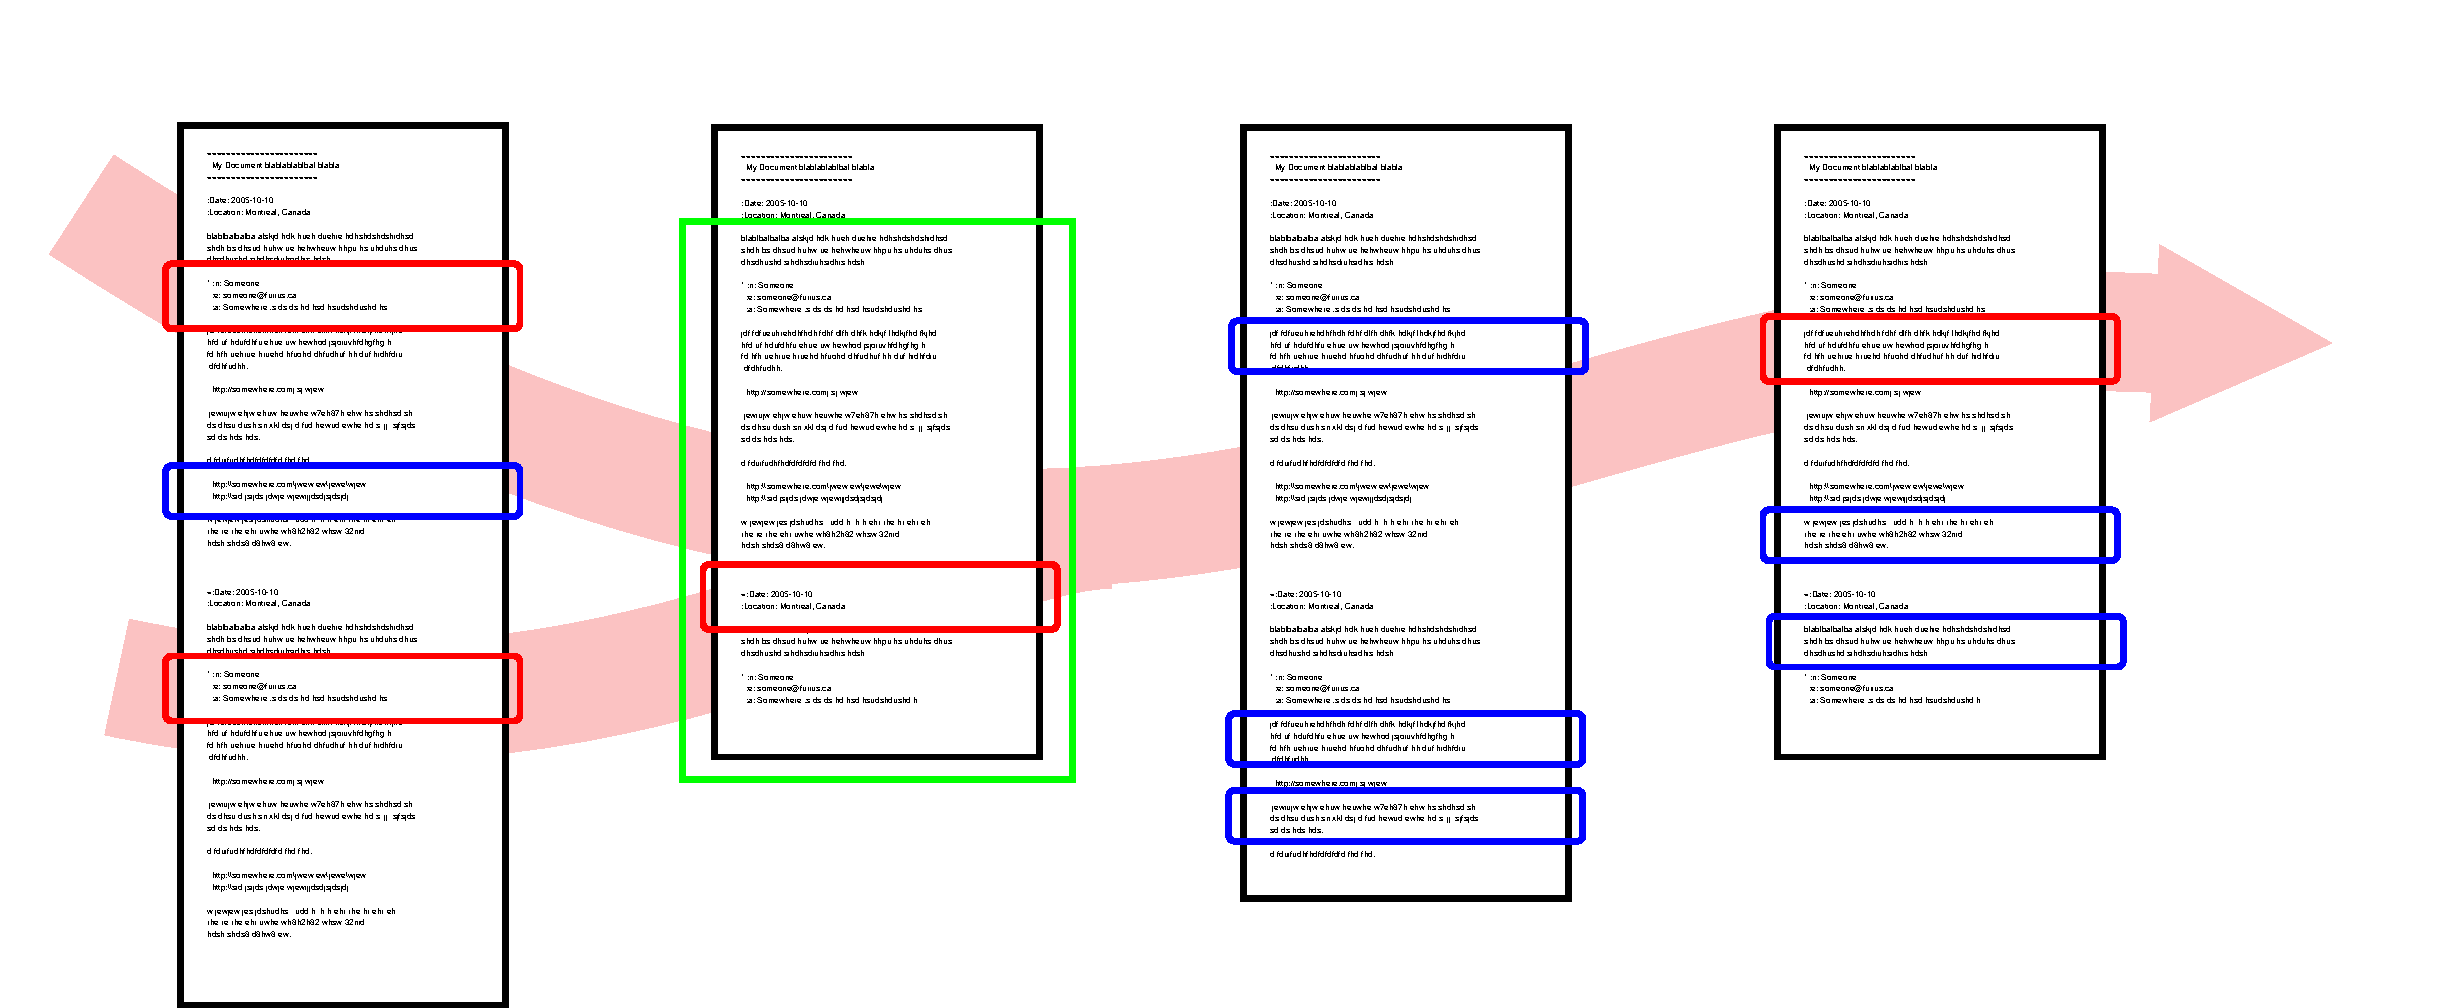
\includegraphics[width=1.0\textwidth]{across3.pdf}

\end{frame}


%-------------------------------------------------------------------------------
\begin{frame}[fragile]
  \frametitle{Data Across Documents}

  What if I could \emph{identify} and \emph{extract} the meaningful parts from
  those files and store them appropriately?  What could I build with this?

\vfill\pause

  Related idea: the Semantic Web
  \begin{itemize}
  \item In an ideal world, web page authors would identify all relevant parts of
    their documents with appropriate markup

  \item You would then be able to collect and use this data, e.g. create an
        ``address book'' of the internet

  \item Search engines are taking a stab at this holy grail

  \end{itemize}

\vfill

  But I want this \textbf{now}, and for just my personal corpus of files, even
  if it's a restricted version of this idea.  I want a database built from the
  files on my computer to feed a website, like a blog on steroids.

\end{frame}


%-------------------------------------------------------------------------------
\begin{frame}[fragile]
  \frametitle{The Goal}

  Build a system that can extract semantically meaningful informations in my set
  of personal info files, using weak heuristics and conventions, and store this
  information in a structured way (in database tables), so I can use this
  information later and serve it in new, interesting ways.

\vfill

  Nabu is a Python library that allows you to do that.
  \begin{itemize}
  \item It is not tied specifically to PIM info
  \item You can write extractors for anything, you just have to establish
    conventions for the docutils structures that you are going to
    recognize/extract
  \item On the client it requires only Python to publish text files \\
    (minimize dependencies to allow easy deployment)
  \end{itemize}

%   If I had served you this definition in the first place, I'm not sure you
%   would be sitting here.

\end{frame}


%-------------------------------------------------------------------------------
\begin{frame}[fragile]
  \frametitle{Components / Overview}

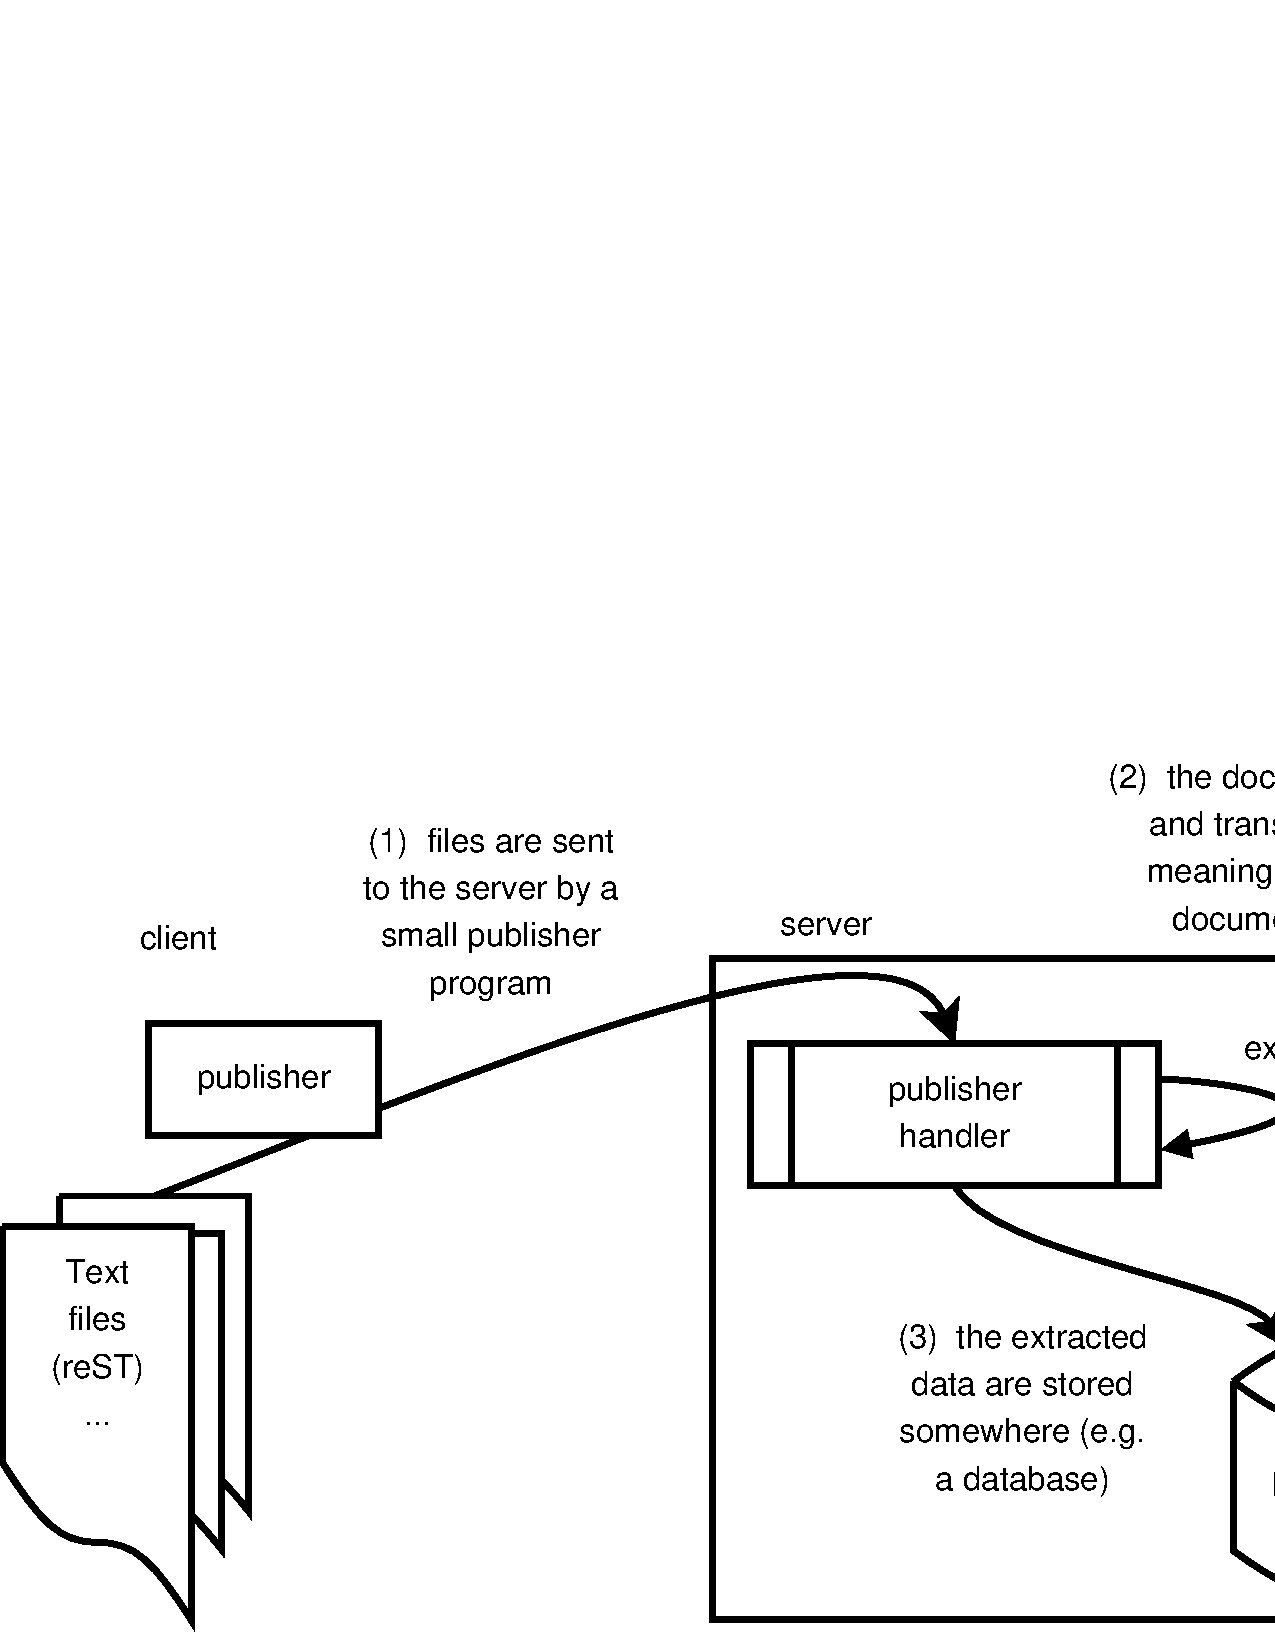
\includegraphics[width=1.0\textwidth]{../nabu2.pdf}

\end{frame}


%-------------------------------------------------------------------------------
\begin{frame}[fragile]
  \frametitle{Components}

  \begin{itemize}
  \item \textbf{Nabu Publisher Client}: searches the files on the client side
    and sends the modified ones to the server
    \begin{itemize}
    \item It fetches MD5 sums from the server and compares the local files
    \item Files are identified by an embedded Id, so file locations don't matter
\begin{verbatim}
   :Id: 8844db51-36ee-4e2a-8255-84e804f5cbe2
\end{verbatim}
    \end{itemize}

\pause
  \item \textbf{Nabu Server}: receives the files, parses them through docutils
    and runs the configured extractors, thereby storing the data
    \begin{itemize}
    \item All extracted data is tagged with the unique id for the file
    \item When a file is uploaded, old data from that file is removed and new
      data replaces it
    \end{itemize}

\pause
  \item \textbf{Storage}: typically, your database server \\
    (or files or anything else if you like)

\pause
  \item \textbf{Presentation}: your own favourite thing \\
     (Nabu does not provide presentation)

  \end{itemize}

\end{frame}


%-------------------------------------------------------------------------------
\begin{frame}[fragile]
  \frametitle{Design}

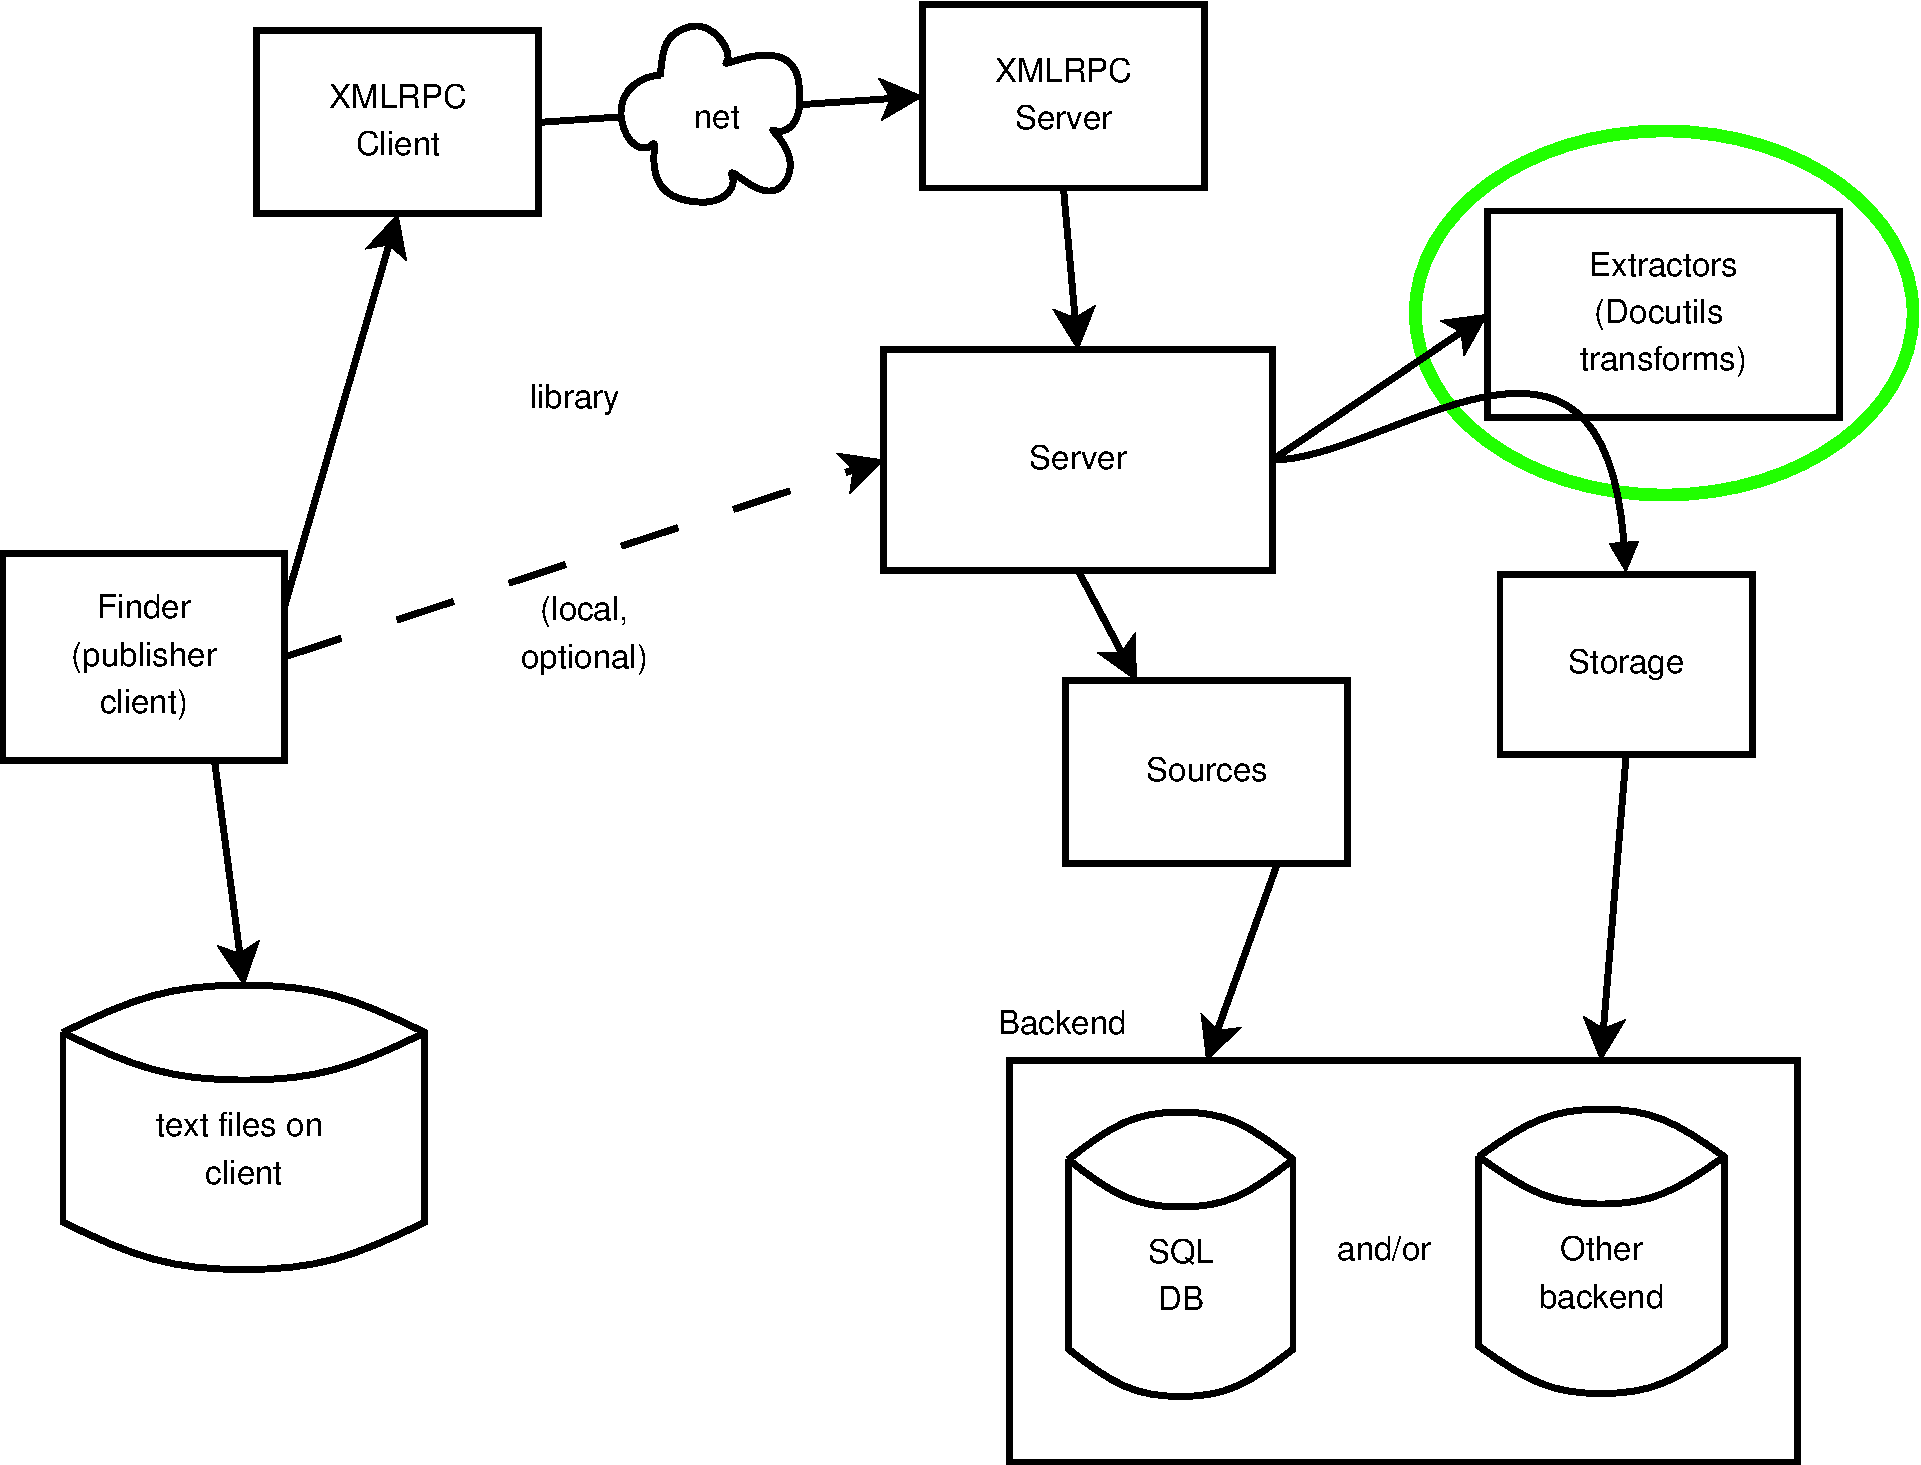
\includegraphics[width=0.9\textwidth]{design.pdf}

\end{frame}


%-------------------------------------------------------------------------------
\begin{frame}[fragile]
  \frametitle{Extractors: Integration with docutils}

  Here is the complete docutils pipeline:

\vfill

  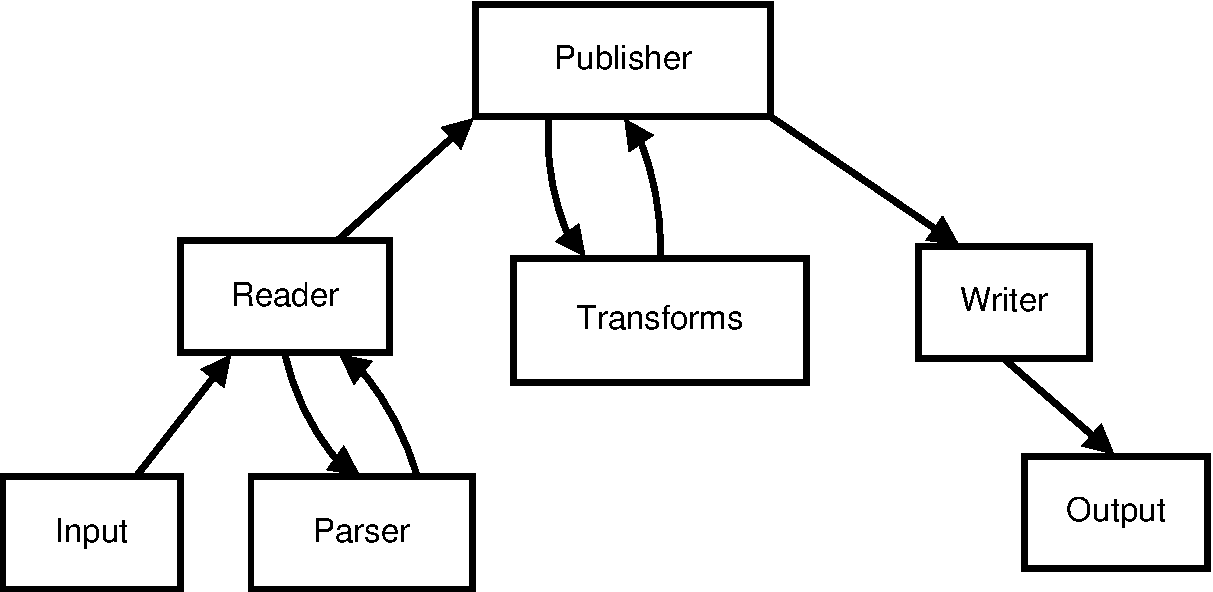
\includegraphics[width=1.0\textwidth]{docutils1.pdf}

\end{frame}


%-------------------------------------------------------------------------------
\begin{frame}[fragile]
  \frametitle{Extractors: Integration with docutils}

  Here is the modified, partial docutils pipeline (no output, just process in
  order to run the extractors):

\vfill

  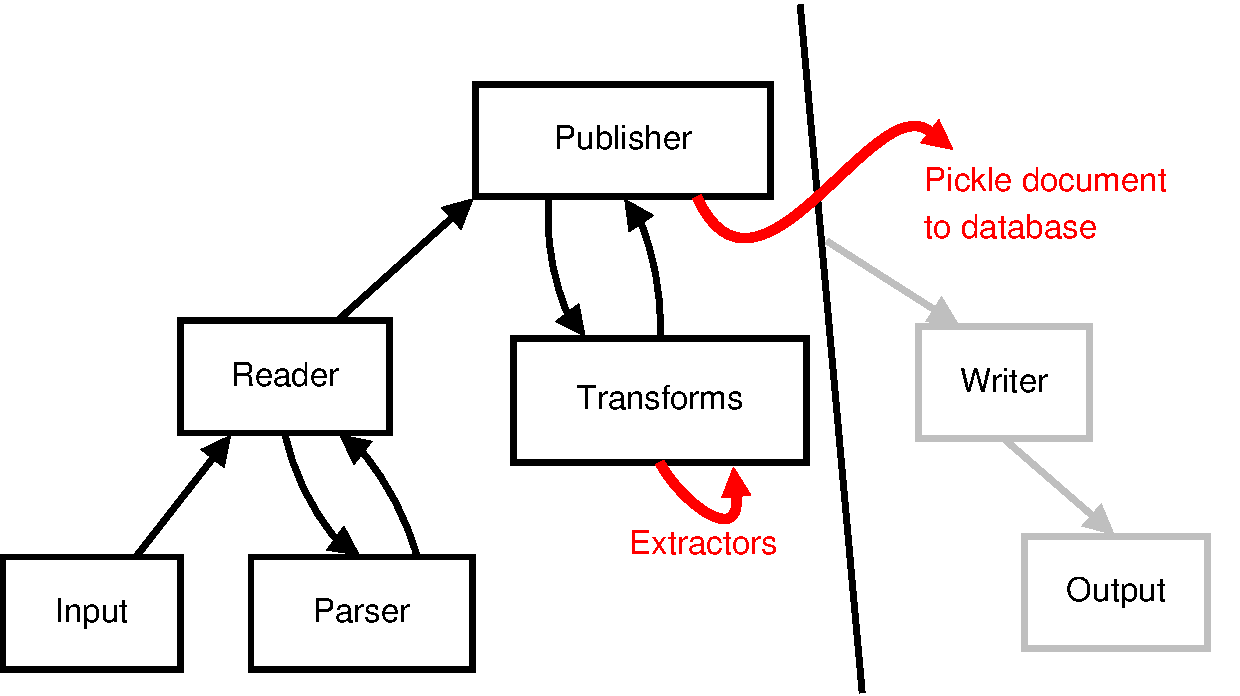
\includegraphics[width=1.0\textwidth]{docutils2.pdf}

\end{frame}


%-------------------------------------------------------------------------------
\begin{frame}[fragile]
  \frametitle{Extractors: docutils document tree}

  \texttt{docutils} is a ``2D parser''
  \begin{itemize}
  \item Its structures are recursive boxes of stuff
  \item For your extractors you have to establish conventions for recognizing
    the stuff you want to extract from your text files
  \end{itemize}

\vfill

\begin{center}
  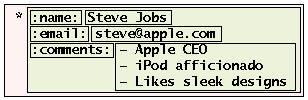
\includegraphics[width=0.8\textwidth]{rest2d.png}

\vfill e.g. has name and (has email or has address)

\end{center}


\end{frame}



%-------------------------------------------------------------------------------
\begin{frame}[fragile]
  \frametitle{Extractors: Viewing the docutils parse tree}

  You need to write extractors for the stuff that you are interested in, for
  example:

{\scriptsize
\begin{verbatim}
     * :name: Bill Gates
       :email: billg@microsoft.com
\end{verbatim}
}

\vfill

  Use \texttt{rst2pseudoxml.py} to figure how docutils parses it:

{\scriptsize
\begin{verbatim}
<bullet_list bullet="*">
    <list_item>
        <field_list>
            <field>
                <field_name>
                    name
                <field_body>
                    <paragraph>
                        Bill Gates
            <field>
                <field_name>
                    email
                <field_body>
                    <paragraph>
                        <reference refuri="mailto:billg@microsoft.com">
                            billg@microsoft.com
\end{verbatim}
}

\end{frame}


%-------------------------------------------------------------------------------
\begin{frame}[fragile]
  \frametitle{Extractors: Implementation}

{\small
Then implement it:
\begin{verbatim}
class AddressExtractor(extract.Extractor):

    def apply( self, **kwargs ):
        v = AddressVisitor(self, self.document)
        self.document.walkabout(v)

class AddressVisitor(...):
    ...

class AddressStorage(extract.SQLExtractorStorage):

    def store( self, unid, name, tfields ):
        ... # store the stuff in a database

\end{verbatim}
%    default_priority = 900
}

\end{frame}


%-------------------------------------------------------------------------------
\begin{frame}[fragile]
  \frametitle{Target Audience}

{\large\begin{center}
\textbf{It's not for your mom!}
\end{center}}

  Nabu is intended only for use by people who have developed the \emph{ability
    to edit text files carefully} (typically programmers, i.e. you guys).

 \begin{itemize}
 \item We understand indentation
 \item We know about spacing, justification, filling, etc.
 \item We are careful about pesky little details
 \item This is what makes creating ReST files possible
 \end{itemize}

\vfill

\begin{center}
  Leverage this ability!
\end{center}

\end{frame}


%-------------------------------------------------------------------------------
\begin{frame}[fragile]
  \frametitle{Presentation: Document Example}

  \begin{center}
    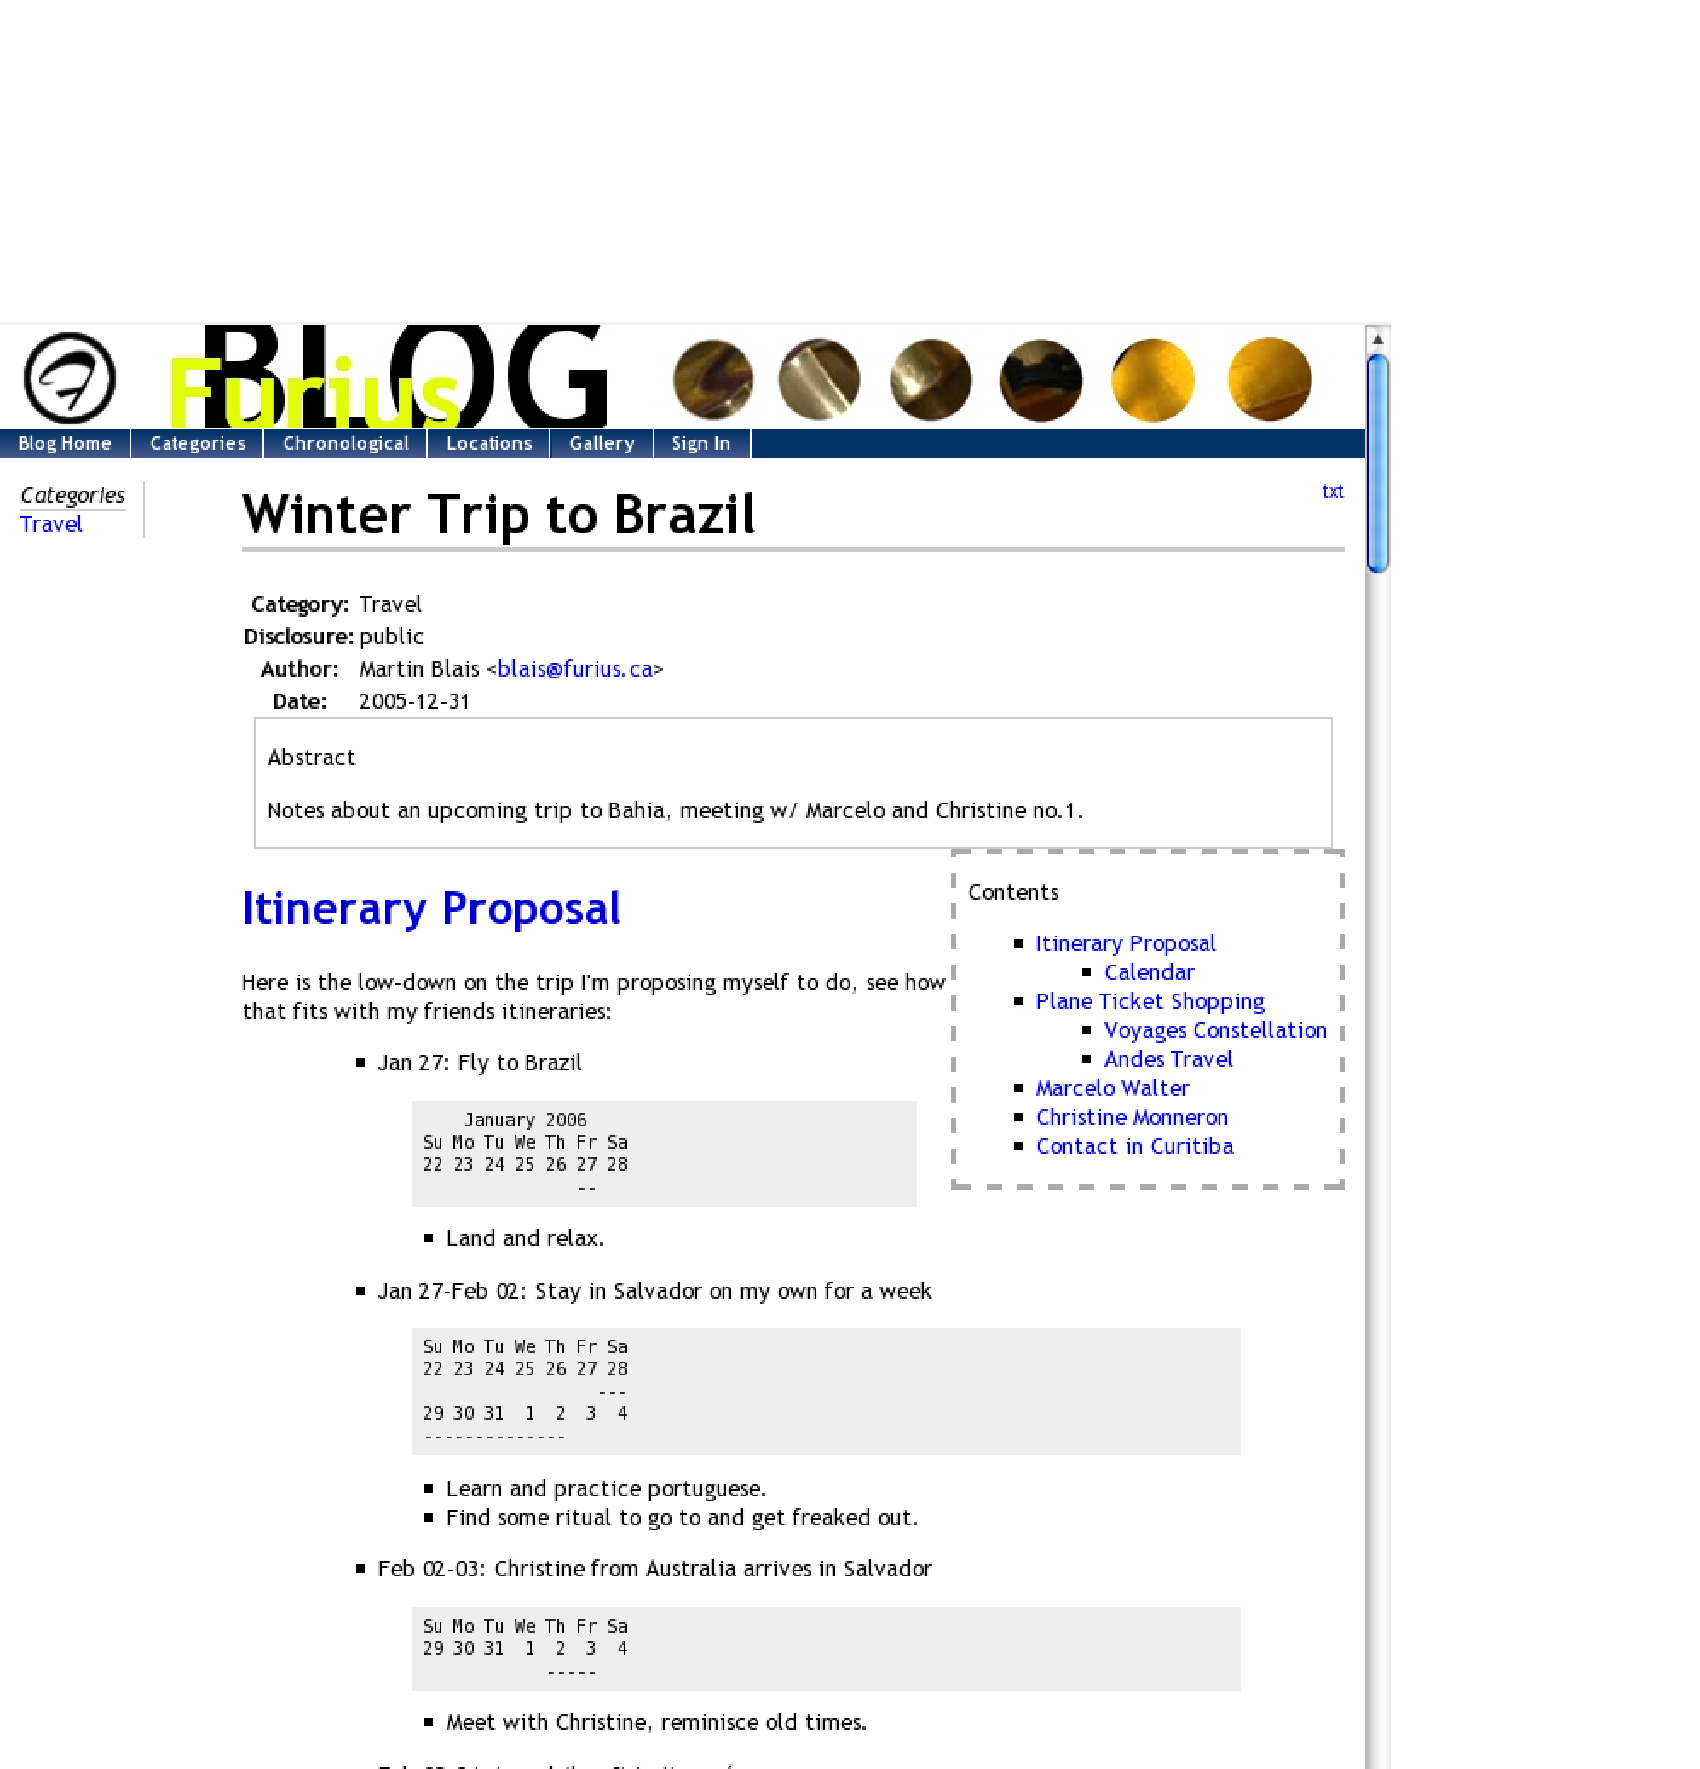
\includegraphics[width=0.9\textwidth]{page-shot.pdf}
  \end{center}

\end{frame}


%-------------------------------------------------------------------------------
\begin{frame}[fragile]
  \frametitle{Presentation: Peepholes}

\vfill

  \begin{center}
    
\includegraphics[width=0.9\textwidth]{peephole1.pdf}
  \end{center}

\vfill
\hrule
\vfill

  \begin{center}
    
\includegraphics[width=0.9\textwidth]{peephole2.pdf}
  \end{center}

\vfill

\end{frame}

%-------------------------------------------------------------------------------
\begin{frame}[fragile]
  \frametitle{Presentation: Peepholes}

  Peepholes are passwordless privileged acccess to selected documents in my Nabu
  store.
  \begin{itemize}
  \item Useful for sending a link to a file that is work-in-progress
  \item Does not require users/passwords, relies on the ``relative'' privacy of
    email
  \item Provides access to only some selected resources
  \item Expires after some time, or after a number of accesses (self-destroying
    links\dots [insert M.I. music here])
  \end{itemize}
\end{frame}


%-------------------------------------------------------------------------------
\begin{frame}[fragile]
  \frametitle{Presentation: Events/Calendar Example}

{\small
\begin{verbatim}
sat 2005-12-31 19h30
  - NYE Evening chez Stuart

sat 2005-12-31
  - Proteus: mkisofs for backup copy DVD-ROM

2006-01-02
  - Contact SonoMax about free earplugs
  - Track Leif's grille that was supposed to arrive.

2006-01-03
  - Visit Yves * D'ailleurs je vais avoir besoin de tes info pour les
    salaires de 2005

  - Confirm flight to Brazil w/ Constellation

2006-01-04 20h00
  - Dinner w/ Pierre @ Golden Cari

2006-01-05
  - Book room for PyCon (should be 79 USD) in january when problems are fixed.

2006-01-13, 14, 16
  - Vote par anticipation

\end{verbatim}
}

\end{frame}


%-------------------------------------------------------------------------------
\begin{frame}[fragile]
  \frametitle{Presentation: Events/Calendar Example}
  \framesubtitle{Calendar View}

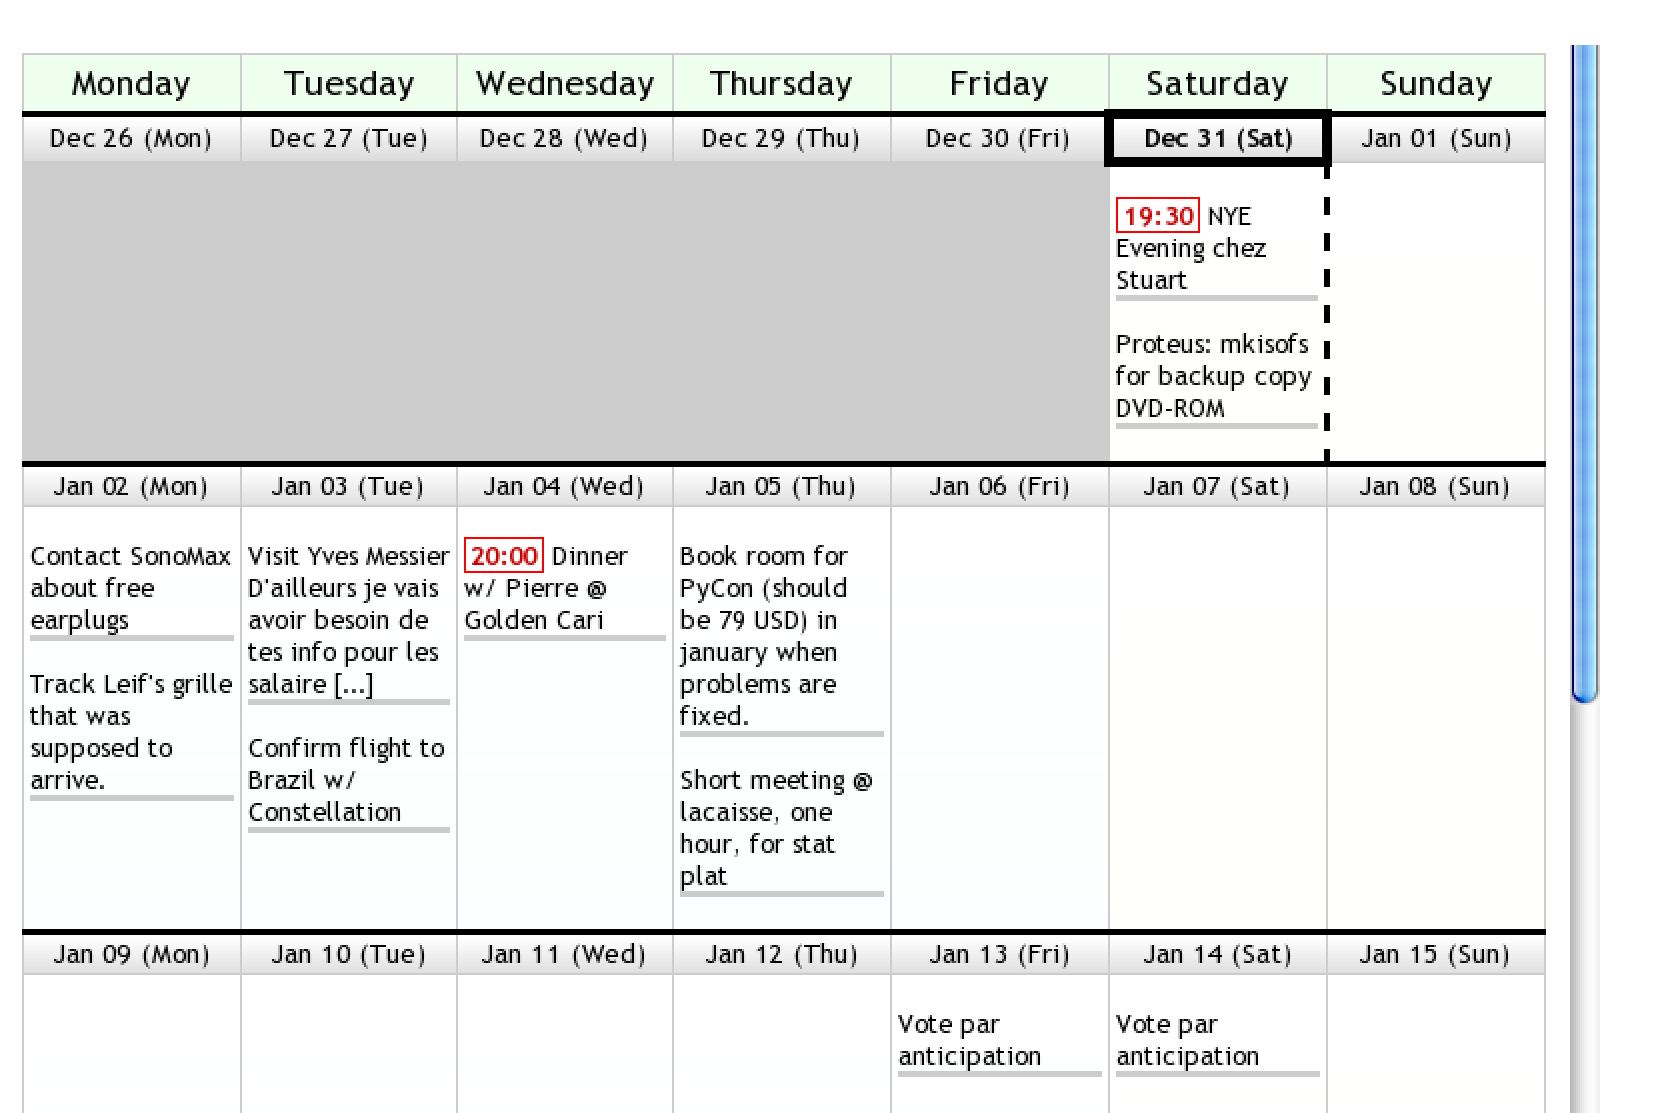
\includegraphics[width=1.0\textwidth]{calendar-shot.pdf}

\end{frame}


%-------------------------------------------------------------------------------
\begin{frame}[fragile]
  \frametitle{Presentation: Other Examples}

  \begin{itemize}
  \item Bookmarks: You can serve your extracted bookmarks from a server using
    RSS format

  \item Billing info: you could define a simple timesheet format in a text file
    and have some kind per-task or per-client billing info page that is always
    up-to-date

  \item Filter all extracted links to Google Maps and generate a map of all of
    the locations with links to the original documents

  \item \dots (insert your own here) \dots

  \item Dynamic website data: you could use Nabu to feed some data for a web
    site, this allows you to \textbf{avoid having to write input forms}

  \end{itemize}

\end{frame}


%-------------------------------------------------------------------------------
\begin{frame}[fragile]
  \frametitle{Debugging: Nabu Contents Browser}
  \framesubtitle{View Uploaded File Details}

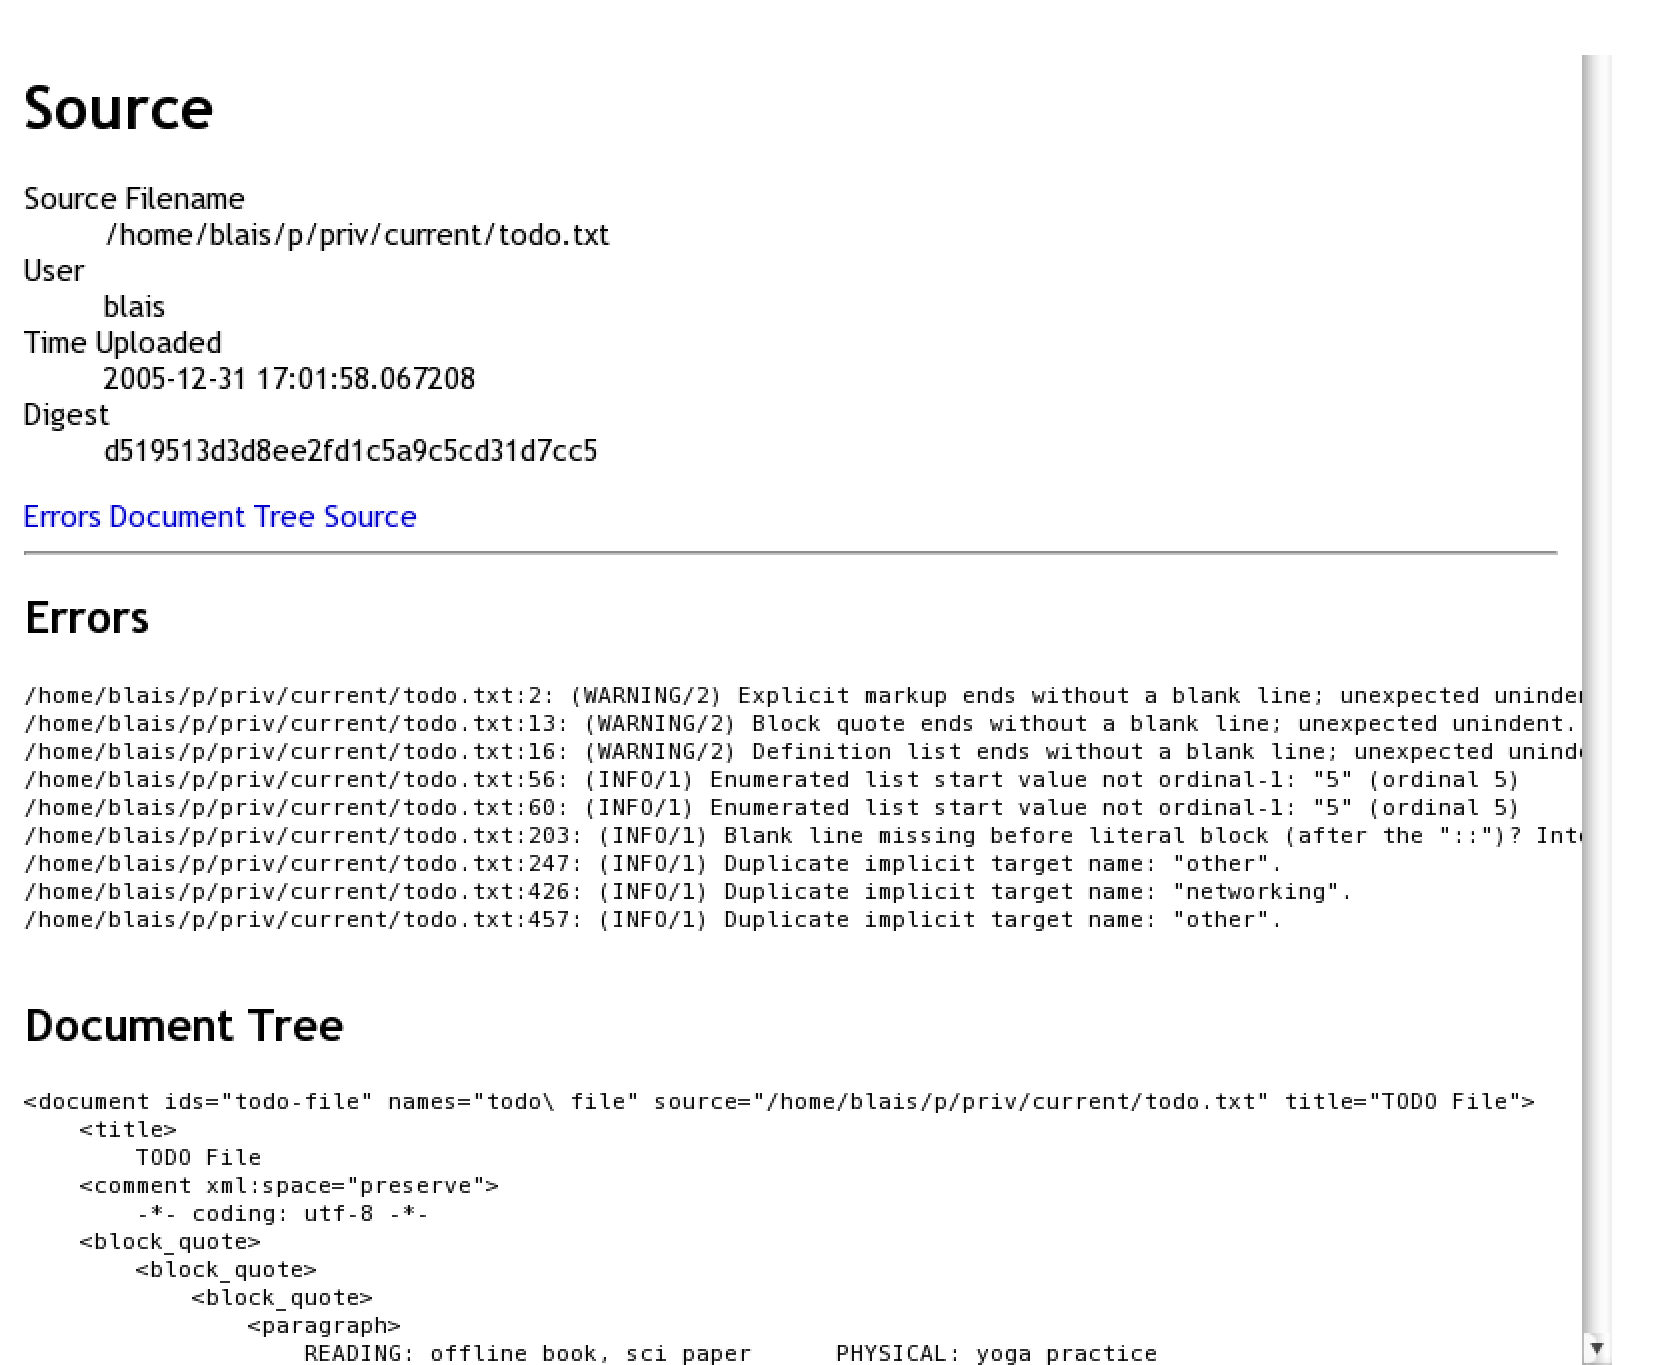
\includegraphics[width=1.0\textwidth]{ll-upload.pdf}

\end{frame}


%-------------------------------------------------------------------------------
\begin{frame}[fragile]
  \frametitle{Debugging: Nabu Contents Browser}
  \framesubtitle{View Extracted Info}

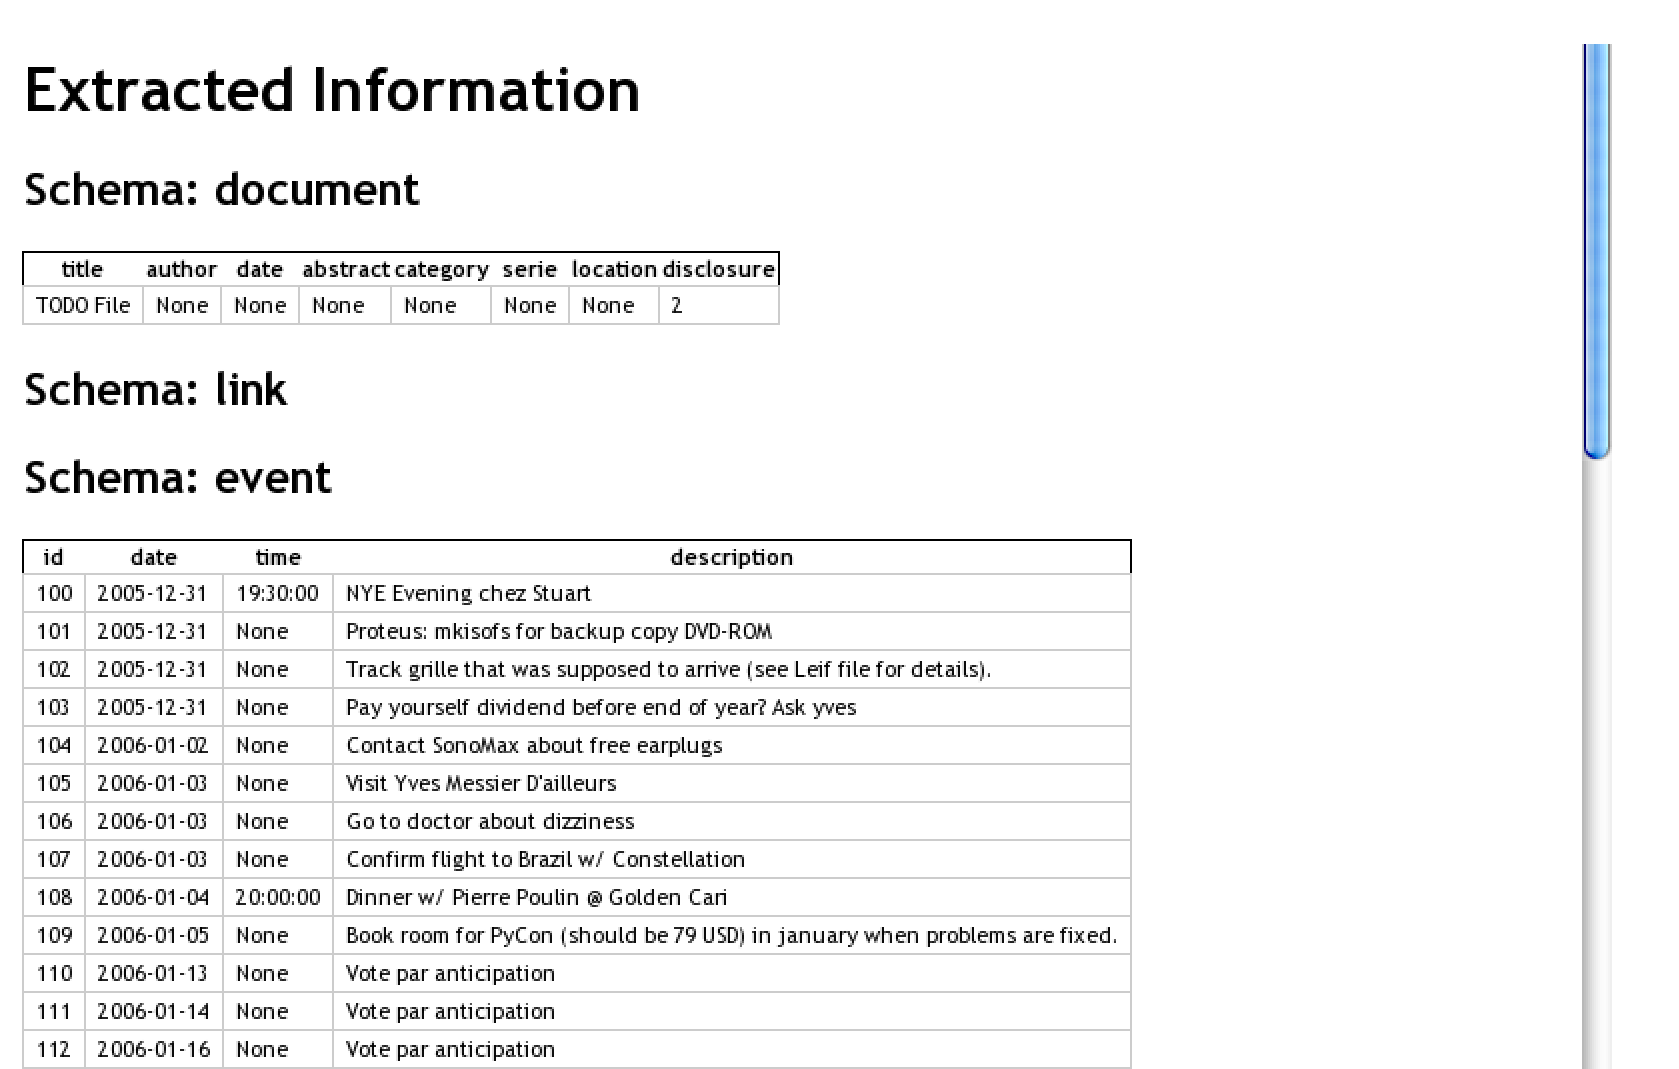
\includegraphics[width=1.0\textwidth]{ll-extracted.pdf}

\end{frame}


%-------------------------------------------------------------------------------
\begin{frame}[fragile]
  \frametitle{Multiple Users}

  There are two approches:

  \begin{enumerate}
  \item Multiple users share a single body of files
    \begin{itemize}
    \item You could update to Nabu on a \textbf{Subversion hook} when files are
      committed
    \end{itemize}

  \item Each user has a distinct body of files
    \begin{itemize}
    \item The Nabu server supports disjoint sets of ids per-user, so that users
      don't have to manually manage avoiding collisions
    \end{itemize}

  \end{enumerate}

\end{frame}



%-------------------------------------------------------------------------------
\begin{frame}[fragile]
  \frametitle{Problems}

  \begin{itemize}
  \item Creating precise reStructuredText can be fragile from the user's
    point-of-view

    \begin{itemize}
    \item You end up having to wrap your head around the docutils document
      structure and knowing ReST really well in order to generate what you need
      (but that is ok)
    \end{itemize}

\vfill

  \item You need to make sure that your set of ids are unique
    \begin{itemize}
    \item I like to use UUIDs like this:
       \verb=  78d8a600-abb4-49c0-a0fc-1c315cddbc1a  =
    \end{itemize}

  \end{itemize}

\end{frame}


%-------------------------------------------------------------------------------
\begin{frame}[fragile]
  \frametitle{Future Work}

  \begin{itemize}

  \item Stabilize more
    \begin{itemize}
    \item I need to write more presentations for my data
    \item Convert presentations output to microformats
    \end{itemize}

  \item Support encryption in the publisher client, hidden files

  \item Support per-document options

  \end{itemize}

\end{frame}


%-------------------------------------------------------------------------------
\begin{frame}[fragile]
  \frametitle{Questions}

  \begin{center}

{\LARGE
Nabu homepage: \\
\verb=http://furius.ca/nabu/=
}

\vfill

Slides will be posted there. \\
I will be around during the sprints.

\vfill

{\LARGE Questions?}

  \end{center}

\end{frame}


%===============================================================================
\end{document}

